\section{Basic Concepts of Federated Learning}
\label{sec:basic}
\subsection{Definition}
Federated Learning~\cite{IEEEstd3652, mcmahan2017communication} is a collaborative machine learning modeling paradigm that enables sharing and aggregation of knowledge from multiple sources while maintaining the confidentiality of source data.
Generally, in terms of task organization, there are two kinds of entities in FL systems: the server and participant. 
The FL server can launche a federated training task and invites participants with sufficient training data and hardware resources to contribute their local modeling results for multi-source knowledge aggregation.
In practice, FL systems can be divided into two categories based on application scenarios~\cite{kairouz2021advances}:
\begin{itemize}
    \item Cross-device FL. In this setting, the participants are numberous end devices with relatively small dataset size, such as mobiles, IoT sensors and wearable devices, the server is hosted in the cloud. Since there is low context correlation between the data of distributed end devices and less overlapping sample ids, this setting typically falls within the scope of horizontal FL. The cross-device FL applications include: Gboard input suggestion~\cite{hard2018federated,ramaswamy2019federated,yang2018applied}, e-commerce recommendation~\cite{niu2020billion}.
    
    \item Cross-silo FL. In this setting, the participants are orginizations or institutions with large amounts of well-maintained structured data, and the server is hosted by a trusted FL service providers such as FATE~\cite{liu2021fate} and NVFLARE~\cite{roth2022nvidia}. As participants can be different departments within an organization, the data silo owned by these departments can have a large overlap in sample space and less overlap in feature space, which falls within vertical FL. The applications of cross-silo FL include federated data analysis for radiomics~\cite{li2019privacy, li2020multi, scherer2020joint}, epidemiology~\cite{dayan2021federated} and EHR~\cite{brisimi2018federated, huang2019patient}.
\end{itemize}

The allocation to the server and participants in FL is dependent on the particular application context. 
Furthermore, FL entities can also serve multiple functional roles to support advanced features such as privacy enhancement~\cite{geyer2017differentially, bonawitz2017practical, niu2020billion}, participant scheduling~\cite{li2022federated, abdulrahman2020fedmccs}, model verification~\cite{tekgul2021waffle, shao2022fedtracker} and incentive mechanisms~\cite{yu2020fairness}.
Recall that there are four roles defined in the FL standard~\cite{IEEEstd3652}:

\begin{itemize}
    \item Model User. The FL model users can request for FL modeling services and preset the targeted task, and then establish cooperation with participants who provide training data. This role can leverage the benefits of collaborative training to improve the preformance of its objective models.
    
    \item Coordinator. The FL coordinators are responsible for providing FL services to all FL entities. This role involves setting up communication channels with entities, initializing the execution environment of participants~\cite{hanzlik2021mlcapsule}, scheduling the training and aggregation workflows for improve system efficiency, such as by alleviating the straggler effect~\cite{li2021fedsae, chai2020tifl}, optimizing data heterogeneity~\cite{duan2019astraea, abdulrahman2020fedmccs} and compressing model transfer~\cite{konevcny2016federated, sattler2019robust}.
    Additionaly, the FL coordinator provides privacy control mechanisms~\cite{bonawitz2017practical, el2022differential, hesamifard2018privacy} for model users and authorization verification for participants to maintain the security of FL systems. 
    Furthermore, the coordinator can hold a validation dataset for evaluate the models contributed by participants or detect potential disturbances from Byzantine attacks~\cite{sattler2020byzantine}.

    \item Data Owner. The FL data owners are knowledge contributors of FL systems, they collect and desentize raw data to maintain a local dataset for federated training. Although they have full authority of data processing and modeling, they cannot share the raw data due to privacy concerns. To address these concerns, de-identification~\cite{act1996health} and differential privacy~\cite{dwork2006differential} techniques can be applied to meet privacy budgets as required by privacy policies.
    
    \item Auditor. The FL auditors are responsible for formulating privacy control policies and establishing supervisory mechanisms that ensure the training process is compliant with data protection regulations (e.g. HIPAA~\cite{act1996health}, GDPR(\cite{voigt2017eu})) and preventing potential privacy breaches for both model users and data owners. Especially in FL, the latent knowledge in models can potentially reveal the sensitive information of training data~\cite{wang2019beyond, zhu2019deep, jin2021cafe}, making it crucial for auditors to scrutinize the model transmission~\cite{wei2021gradient, li2022auditing} and verify the ownership of models~\cite{tekgul2021waffle, shao2022fedtracker}.
\end{itemize}

\begin{figure}[t]
    \centering
    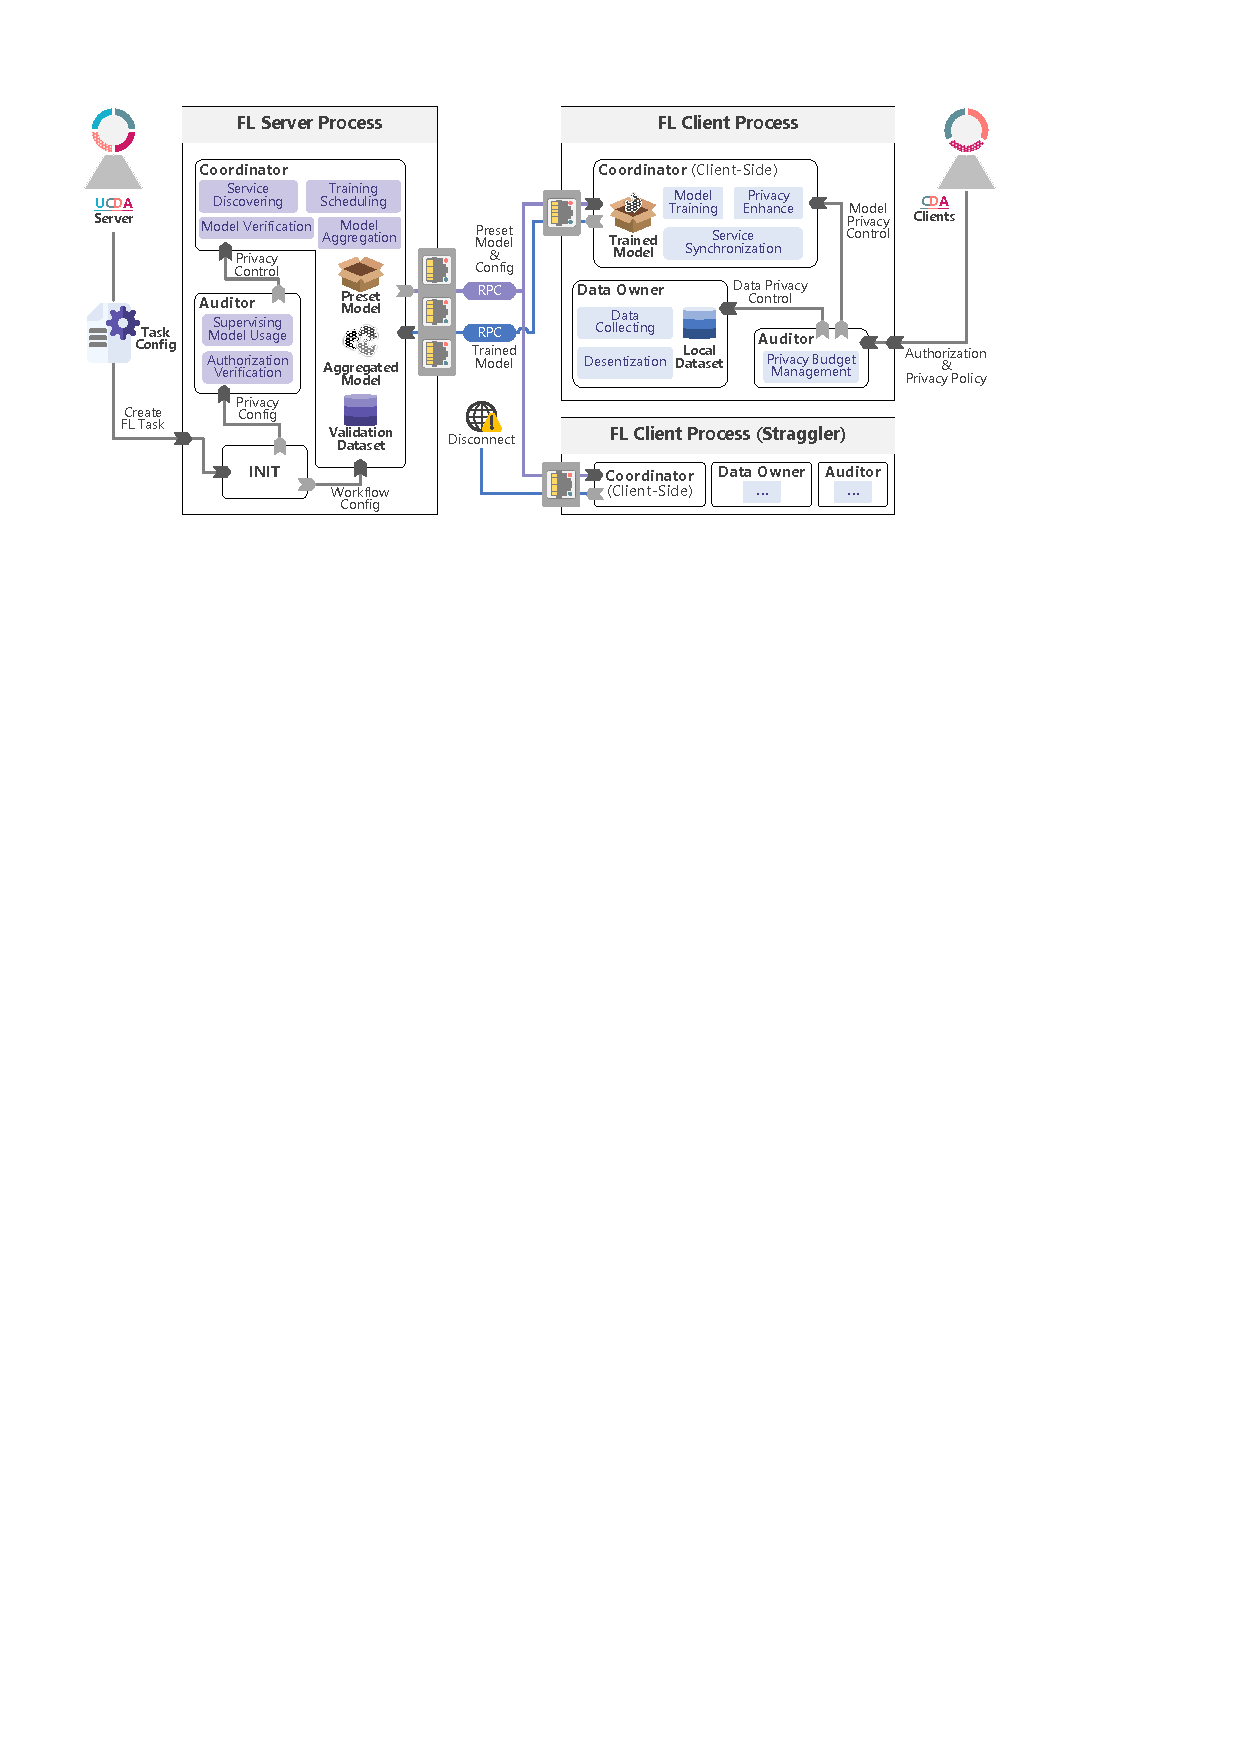
\includegraphics[width=\linewidth]{fig/fl_frame.pdf}
    \caption{An overview of traditional FL systems. (U: model User, C: Coordinator, D: Data owner, A: Auditor)}
    \Description{}
    \label{fig:fl}
  \end{figure}

Fig.~\ref{fig:fl} illustrates the typical architecture of FL systems, which as a distributed modeling toolkits consists of server part and client part. In general FL setting, the server part is the central aggregator installed in a trusted cloud environment, while the client part of software can operate in different operating environments of client devices. 
The server and clients are connected via Internet and typically with the help of Remote Procedure Call (RPC) interface for coordinating~\cite{zhang2022felicitas, abadi2016tensorflow, liu2021fate, beutel2020flower, he2020fedml}.
We use four colors to represent the four FL roles and the colors with grid lines indicate non-essential roles.
For example, in Fig.~\ref{fig:fl}, the UCDA server takes on the roles of model user, coordinator and audior in traditional FL. 
However, it is no necessary to hold training data or validation data, so the role of data owner is non-essential.
To illustrate the workflow of traditional FL, we leverage the vanilla FL framework Federated Averaging (FedAvg)~\cite{mcmahan2017communication, bonawitz2019towards} as an example.

First, the FL server pre-defines the objective modeling task and initializes the server process.
Secondly,  the coordinator in server-side specifies a preset global model and the operational parameters.
Thirdly, the coordinator discovers the availability of clients' FL services, boardcasts the global model and training config to them. The training config contains bath size, local epoch round, optimizer parameters and so on. Then, the coordinator will wait for the trained results contributed by the coordinator in clients-side and drop those clients with network problems.
Finally, the server aggregates the trained resultes received from various clients into the global model and begins a new round based on this aggregated global model. 
The aggregation strategy adopted in FedAvg is the weighted model parameters based on the size of local dataset, which means the global objective of FL can be regarded as a joint objective function of clients. 
By this way, the FL server can learn a generalized global model by jointly optimizing all local optimization objectives and incorporating the latent knowledge from the local models.
Although the auditor component was not included in earlier FedAvg, it play an important role in the later business-ready FL frameworks~\cite{liu2021fate,roth2022nvidia, ziller2021pysyft}.

However, in comparing FedAvg workflow described above with Fig.~\ref{fig:fl}, it is easy to notice that the client part has been excluded.
This is because we are elaborating from a server-side perspective, which is usual way FL is presented~\cite{mcmahan2017communication, li2020ditto, caldas2018leaf}.
Actually, the underlying reason is that in traditional FL, the client-side process is tightly coupled with server-side process, and there is no alternative for clients other than to either accept or reject the training scheduling from the server wholesale.
So the clients are not considered as an autonomous entities but rather work as subordinates to server.
In this server-domianted cooperation framework, the benefits and autonomy of clients are compromised, which hinders their enthusiasm to participate in FL network and subsequently limits the applicability of FL.
From this perspective, we summarize the limitations of traditional FL in the next section, which motivates us to explore more innovative sustainable FL cooperation frameworks.

\subsection{Limitations of Traditional FL}
Previous surveys~\cite{kairouz2021advances, zhang2022federated, alazab2021federated, nguyen2021federated, zhu2022blockchain, li2020federated, yang2019federated, tan2022towards} has extensively discussed the challenges in FL systems from various aspects
However, the cooperation mechanism of FL systems has been overlook because almost all mainsteam FL frameworks follow the FL prototype~\cite{mcmahan2017communication}, which shape the form of current FL frameworks: a modeling software.
We summarize three inherent limitations of traditional FL cooperation mechanism: (1) \textbf{Server-client Coupling}, (2) \textbf{Low Model Reusability}, (3) \textbf{Non-public}.

\subsubsection{Server-client Coupling} 
% 设备异构 从客户端层面,从服务端层面
% 不合理假设,稳定的链接和已经安装好了软件(侵入式的,后台运行,损害客户端的独立性,恶意软件,资源浪费
The tightly-coupled server-client design is a major limitation of FL systems. From the perspective of FL service providers, adapting the programs to heterogeneous client hardware and software components, such as various operating and database systems, processor and storage architectures, communication protocols, eneragy constrains and data licenses, is a challenging task that significantly increases the complexity of the FL system. 
    
On the other hand, the invasive software deploy mode compromises the integrity of client environments and expose them to new privacy risks.
Specifically, the coordinator components (client-side) pushed by the server may not offer demanded privacy control mechanisms~\cite{zeng2021fedlab, caldas2018leaf, mcmahan2017communication}, or cause resource depletion on client-side~\cite{bonawitz2019towards, niu2020billion, chen2020deep}, or even piggyback malicious executable codes~\cite{li2017understanding}.
So the auditor role of client is non-essential as depicted in Fig.~\ref{fig:fl}, not only because the client maybe lacks a corresponding policy for FL training, but also because its privacy is not completely under its control.
Likewise, the malicious clients can also exploit the vulnerability in the aggreagation strategy to currupt the FL tranining process~\cite{bouacida2021vulnerabilities, sattler2020byzantine, park2021sageflow, fang2020local} or insert backdoors~\cite{bagdasaryan2020backdoor, wang2020attack}.
In addition, the unstable network environment can drive clients to drop out from traning (i.e. straggler effect), thereby reducing system efficiency~\cite{reisizadeh2019robust, park2021sageflow}.
Therefore, the server-client coupling design of traditional FL systems make them susceptible to unpredictable runtime environments, leading to system vulnerability and low reliability.

\subsubsection{Low Model Reusability} % 模型的移植性 不可持续 模型的可发现性
The traditional FL scheduling follows a task-centric manner and erminates once the training reaches a preset number of rounds or meets traget metrics on global model set by FL server~\cite{bonawitz2019towards}.
As a result, only FL server can guarantee having the latest global model after the task is terminated.
This ad-hoc modeling paradigm results in low model reusability and transportability.
For example, if a client who participated in the previous training turn wants to continue training, they can only start the task from scratch unless they have the up-to-date global model.
Since only FL server is able to maintain the complete modeling trajectory, it is difficult for the client to roll back the training itself to eliminate the potential privacy risk.
Furthermore, the non-deliverable scheduling mechanism of FL tasks also hinders inter-task model reuse, which leads to unnecessary wasted energy and time on participants that have been involved in similar tasks.

\subsubsection{Non-public} % 无法自由发起任务,不提供公共接口
As we mention in Sec.~\ref{sec:flsystems}, except PySyft~\cite{ziller2021pysyft}, the application scenarios of mainstream FL frameworks~\cite{liu2021fate, abadi2016tensorflow, zeng2021fedlab, caldas2018leaf, ibmfl2020ibm, he2020fedml, beutel2020flower, roth2022nvidia} aim to provide private collaborative ML traning service, and there is no any accessible FL platform for the public.
Although there have been real-world deployment practices of FL for the public with scales of millions~\cite{bonawitz2019towards} and billions~\cite{niu2020billion}, these have been carried out only by tech giants with a massive base of active users. For an individual user, there is no practical way to organize such a large-scale FL training network.

But in fact, due to the limitations in the cooperation mechanism mentioned above, data owners are not sufficiently motivated to participate in this server-take-all FL training even if it is public accessible. Therefore, the cornerstone of buliding a sustainable open FL platform is to establish a reciprocal FL cooperation framework, followed by corresponding multi-source knowledge aggregation strategies, which we discuss in the following sections.